\documentclass[a4paper]{exam}

\usepackage{xcolor}
\usepackage{geometry}
\usepackage{graphicx}
\usepackage{hyperref}
\usepackage{mathtools}
\usepackage{titling}
\usepackage{amssymb}
\usepackage{amsmath}
\usepackage{amsthm}
\usepackage{mdframed}
\usepackage{amsfonts}
\usepackage{geometry}
\usepackage{hyperref}
\usepackage{forest}
\usepackage{tikz} 
\usepackage{tikz-qtree}

\definecolor{ocre}{RGB}{243,102,25}
\definecolor{mygray}{RGB}{243,243,244}
\definecolor{deepGreen}{RGB}{26,111,0}
\definecolor{shallowGreen}{RGB}{235,255,255}
\definecolor{deepBlue}{RGB}{61,124,222}
\definecolor{shallowBlue}{RGB}{235,249,255}

\newcommand\orangebox[1]{\fcolorbox{ocre}{mygray}{\hspace{1em}#1\hspace{1em}}}

\newtheoremstyle{mytheoremstyle}{3pt}{3pt}{\normalfont}{0cm}{\rmfamily\bfseries}{}{1em}{{\color{black}\thmname{#1}~\thmnumber{#2}}\thmnote{\,--\,#3}}
\newtheoremstyle{myproblemstyle}{3pt}{3pt}{\normalfont}{0cm}{\rmfamily\bfseries}{}{1em}{{\color{black}\thmname{#1}~\thmnumber{#2}}\thmnote{\,--\,#3}}
\theoremstyle{mytheoremstyle}
\newmdtheoremenv[linewidth=1pt,backgroundcolor=shallowGreen,linecolor=deepGreen,leftmargin=0pt,innerleftmargin=20pt,innerrightmargin=20pt,]{theorem}{Theorem}[]
\theoremstyle{mytheoremstyle}
\newmdtheoremenv[linewidth=1pt,backgroundcolor=shallowBlue,linecolor=deepBlue,leftmargin=0pt,innerleftmargin=20pt,innerrightmargin=20pt,]{definition}{Definition}[]
\theoremstyle{myproblemstyle}
\newmdtheoremenv[linecolor=black,leftmargin=0pt,innerleftmargin=10pt,innerrightmargin=10pt,]{problem}{Problem}[]

\printanswers

\title{Weekly Challenge 05: Master Theorem\\CS 412 Algorithms: Design and Analysis}
\author{q1-team-2}  % <==== replace with your team name for grading
\date{Habib University | Spring 2023}

\runningheader{CS 412: Algorithms}{WC05: Master Theorem}{\theauthor}
\runningheadrule
\runningfootrule
\runningfooter{}{Page \thepage\ of \numpages}{}

\qformat{{\large\bf \thequestion. \thequestiontitle}\hfill}
\boxedpoints

\begin{document}
\maketitle

\begin{questions}


	\titledquestion{Reverse Engineering}

	We are going to design algorithms to meet a target asymptotic time complexity, and then investigate their running time.

	\subsection*{Tasks}
	\begin{description}
		\item[Theorem] State the master theorem.
		\item[Recurrences 1] Design distinct recurrences, $T_A(n)$ and $T_B(n)$, each of which solve to $\Theta(n^2)$.
		\item[Recurrences 2] Design distinct recurrences, $T_C(n)$ and $T_D(n)$, each of which solve to $\Theta(n\lg n)$.
		\item[Justify] Use the master theorem to justify the claimed solutions of  $T_A(n)$, $T_B(n)$, $T_C(n)$, and $T_D(n)$.
		\item[Solve 1] Use any other method to solve any one of  $T_A(n)$ and $T_B(n)$.
		\item[Solve 2] Use any other method to solve any one of  $T_C(n)$ and $T_D(n)$.
		\item[Implement 1] In the accompanying file, \texttt{algos.py}, implement plausible algorithms whose running times match $T_A(n),T_B(n), T_C(n)$, and $T_D(n)$. You may modify the parameter list of each as required.
		\item[Timing] Time the run time of your 4 algorithms In the accompanying file, \texttt{algos.py}, across a wide range of values of $n$.
		\item[Compare] Plot the run time of your algorithms in a single diagram. Make sure that each plot is clearly labeled, or the diagram contains a clearly visible legend. Make sure that the axis limits are set such that the plots are clearly visible and occupy a large portion of the diagram. Include separate diagrams over different axis ranges for greater clarity if necessary.
		\item[Submit] Include the diagram in your solution below.
		\item[Share] Share your diagram as a comment on the \href{https://web.yammer.com/main/org/habib.edu.pk/threads/eyJfdHlwZSI6IlRocmVhZCIsImlkIjoiMjEyMzI4NzkzMzY4MTY2NCJ9}{WC05 post} in the course group.
	\end{description}
	\underline{Tip}: You may consider \href{https://stackoverflow.com/a/68054319/1382487}{\texttt{time.perf\_counter()}} (detailed tutorial \href{https://realpython.com/python-timer/#other-python-timer-functions}{here}) for timing purposes.

	\begin{solution}
		The general version of the Master Theorem is:
		\begin{theorem}[Master Theorem]
			Let \(a>0\) and \(b>1\) be constants, and let \(f(n)\) be a driving function that is deûned and nonnegative on all sufficiently large reals. Define the recurrence \(T(n)\) on \(n\in\mathbb{N}\) by
			\[
				T(n) = aT\left(\frac{n}{b}\right)+f(n)
			\]
			where \(\displaystyle aT\left(\frac{n}{b}\right)\) actually means \(\displaystyle a'T\left(\left\lfloor\frac{n}{b}\right\rfloor\right)+a''T\left(\left\lceil\frac{n}{b}\right\rceil\right)\) for some constants \(a' \geq 0\) and \(a'' \geq 0\) satisfying \(a = a' + a''\). Then the asymptotic behavior of \(T(n)\) can be characterized as follows:
			\begin{enumerate}
				\item \[\exists \varepsilon > 0 \ni f(n) = O\left(n^{\log_b{(a)}-\varepsilon}\right)\implies T(n)=\Theta\left(n^{\log_b{(a)}}\right)\]
				\item \[\exists k \geq 0 \ni f(n) = \Theta\left(n^{\log_b{(a)}}\lg^k(n)\right) \implies T(n)=\Theta\left(n^{\log_b{(a)}}\lg^{k+1}(n)\right)\]
				\item \begin{multline*}
					      \left(\exists \varepsilon > 0 \ni f(n) = \Omega\left(n^{\log_b{(a)}+\varepsilon}\right)\right)\land \\
					      \left( \exists c<1\ni af\left(\frac{n}{b}\right) \leq cf(n) \right) \implies T(n)=\Theta\left(f(n)\right)
				      \end{multline*}
			\end{enumerate}
		\end{theorem}
		The special case version of the Master Theorem is that we will be using is:
		\begin{theorem}[Master Theorem]
			Let $T(n) = aT\left(\frac{n}{b}\right) + \Theta(n^d)$ be recurrence relation where $a > 0$, $b > 1$, and $d \geq 0$ then,
			$$T(n) = \begin{cases}
					\Theta(n^d) \text{ if } d > \log_ba\\
					\Theta(n^d \lg n) \text{ if } d = \log_ba\\
					\Theta(n^{\log_ba}) \text{ if } d < \log_ba
			\end{cases}$$

		\end{theorem}
		\textbf{Recurrences 1:}
		$$T_A(n) = 2T_A\left(\frac{n}{2}\right) + \Theta(n^2),\text{ where } T_A(1) = C_1$$
		$$T_B(n) = 4T_B\left(\frac{n}{2}\right) + \Theta(n),\text{ where } T_B(1) = C_2$$
		\textbf{Recurrences 2:}
		$$T_C(n) = 2T_C\left(\frac{n}{2}\right) + \Theta(n),\text{ where } T_C(1) = C_3$$
		$$T_D(n) = 4T_D\left(\frac{n}{4}\right) + \Theta(n),\text{ where } T_D(1) = C_4$$
		\textbf{Justification:}
		\begin{itemize}
			\item \textbf{For $T_A(n)$ :}
				$$d = 2,\;\; a = 2,\;\;b=2 \text{ as } d > \log_ba \text{ then } T_A(n) = \Theta(n^d) = \Theta(n^2)$$
			\item \textbf{For $T_B(n)$ :}
				$$d = 1,\;\; a = 4,\;\;b=2 \text{ as } d < \log_ba \text{ then } T_A(n) = \Theta(n^{\log_ba}) = \Theta(n^2)$$
			\item \textbf{For $T_C(n)$ :}
				$$d = 1,\;\; a = 2,\;\;b=2 \text{ as } d = \log_ba \text{ then } T_A(n) = \Theta(n^d \lg n) = \Theta(n \lg n)$$
			\item \textbf{For $T_D(n)$ :}
				$$d = 1,\;\; a = 4,\;\;b=4 \text{ as } d = \log_ba \text{ then } T_A(n) = \Theta(n^d \lg n) = \Theta(n \lg n)$$
		\end{itemize}
		\textbf{Solve 1:}
		\\We will use recursion tree method to solve $T_B(n)$
		$$T_B(n) = 4T_B\left(\frac{n}{2}\right) + \Theta(n)$$
		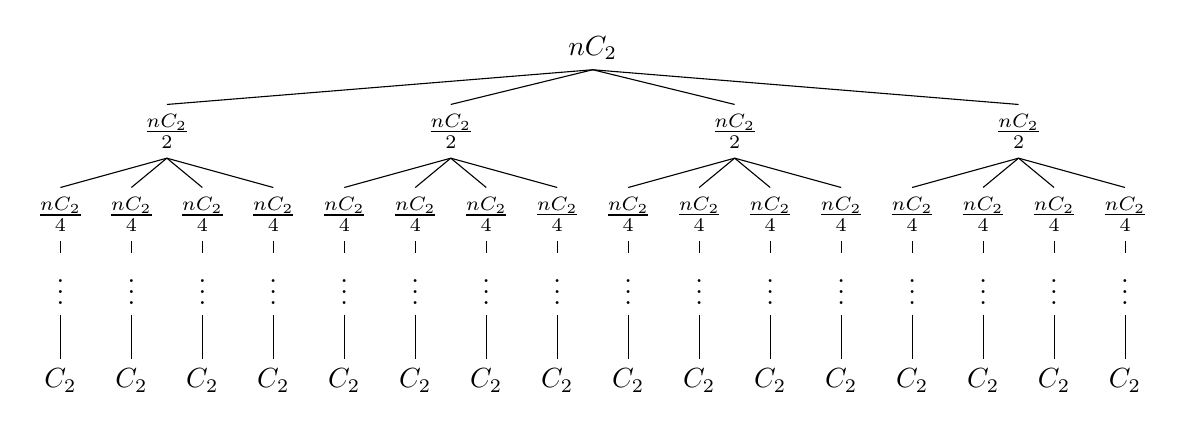
\begin{tikzpicture}
			\Tree [.\node{$nC_2$};
			[.\node{$\frac{nC_2}{2}$};
			[.\node{$\frac{nC_2}{4}$};
			[.\node{\vdots};[.\node{$C_2$};]
			]
			]
			[.\node{$\frac{nC_2}{4}$};
			[.\node{\vdots};[.\node{$C_2$};]
			]
			]
			[.\node{$\frac{nC_2}{4}$};
			[.\node{\vdots};[.\node{$C_2$};]
			]
			]
			[.\node{$\frac{nC_2}{4}$};
			[.\node{\vdots};[.\node{$C_2$};]
			]
			]
			]
			[.\node{$\frac{nC_2}{2}$};
			[.\node{$\frac{nC_2}{4}$};
			[.\node{\vdots};[.\node{$C_2$};]
			]
			]
			[.\node{$\frac{nC_2}{4}$};
			[.\node{\vdots};[.\node{$C_2$};]
			]
			]
			[.\node{$\frac{nC_2}{4}$};
			[.\node{\vdots};[.\node{$C_2$};]
			]
			]
			[.\node{$\frac{nC_2}{4}$};
			[.\node{\vdots};[.\node{$C_2$};]
			]
			]
			]
			[.\node{$\frac{nC_2}{2}$};
			[.\node{$\frac{nC_2}{4}$};
			[.\node{\vdots};[.\node{$C_2$};]
			]
			]
			[.\node{$\frac{nC_2}{4}$};
			[.\node{\vdots};[.\node{$C_2$};]
			]
			]
			[.\node{$\frac{nC_2}{4}$};
			[.\node{\vdots};[.\node{$C_2$};]
			]
			]
			[.\node{$\frac{nC_2}{4}$};
			[.\node{\vdots};[.\node{$C_2$};]
			]
			]
			]
			[.\node{$\frac{nC_2}{2}$};
			[.\node{$\frac{nC_2}{4}$};
			[.\node{\vdots};[.\node{$C_2$};]
			]
			]
			[.\node{$\frac{nC_2}{4}$};
			[.\node{\vdots};[.\node{$C_2$};]
			]
			]
			[.\node{$\frac{nC_2}{4}$};
			[.\node{\vdots};[.\node{$C_2$};]
			]
			]
			[.\node{$\frac{nC_2}{4}$};
			[.\node{\vdots};[.\node{$C_2$};]
			]
			]
			]
			]
			\end{tikzpicture}-2
		\\Here on level 1 the amount of work is $nC_2$, on level 2 the amount of work is $\frac{4nC_2}{2} = 2nC_2$, 
		on level 3 the amount of work is $\frac{16nC_2}{4} = 4nC_2$ and so on, there are total of $\log_2n$ levels.
		\\So the total work is, 
		$$T_B(n) = \sum\limits_{i=0}^{\log_2n}2^inC_2 = C_2n\sum\limits_{i=0}^{\log_2n}2^i = C_2n(2n-1) = \Theta(n^2)$$
		\textbf{Solve 2:}
		\\We will use recursion tree method to solve $T_C(n)$
		$$T_C(n) = 2T_C\left(\frac{n}{2}\right) + \Theta(n)$$
		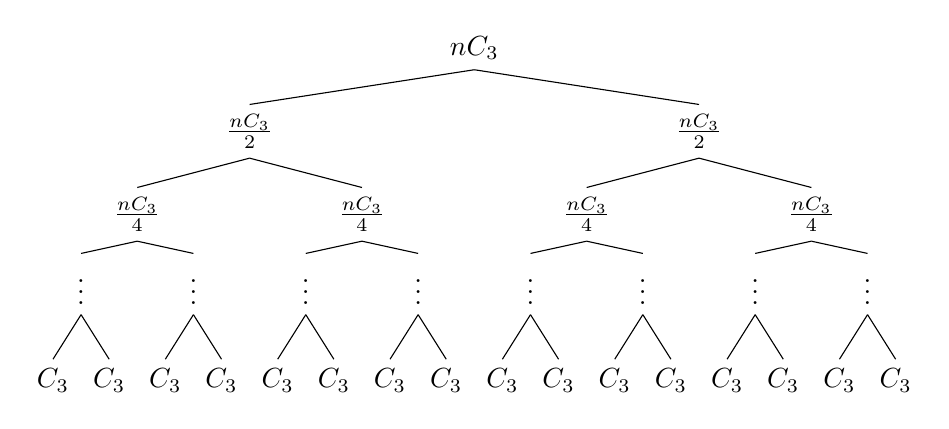
\begin{tikzpicture}
			\Tree [.\node{$nC_3$};
			[.\node{$\frac{nC_3}{2}$};
			[.\node{$\frac{nC_3}{4}$};
			[.\node{\vdots};
			[.\node{$C_3$};
			]
			[.\node{$C_3$};
			]
			]
			[.\node{\vdots};
			[.\node{$C_3$};
			]
			[.\node{$C_3$};
			]
			]
			]
			[.\node{$\frac{nC_3}{4}$};
			[.\node{\vdots};
			[.\node{$C_3$};
			]
			[.\node{$C_3$};
			]
			]
			[.\node{\vdots};
			[.\node{$C_3$};
			]
			[.\node{$C_3$};
			]
			]
			]
			]
			[.\node{$\frac{nC_3}{2}$};
			[.\node{$\frac{nC_3}{4}$};
			[.\node{\vdots};
			[.\node{$C_3$};
			]
			[.\node{$C_3$};
			]
			]
			[.\node{\vdots};
			[.\node{$C_3$};
			]
			[.\node{$C_3$};
			]
			]
			]
			[.\node{$\frac{nC_3}{4}$};
			[.\node{\vdots};
			[.\node{$C_3$};
			]
			[.\node{$C_3$};
			]
			]
			[.\node{\vdots};
			[.\node{$C_3$};
			]
			[.\node{$C_3$};
			]
			]
			]
			]
			]
			\end{tikzpicture}
		\\Here on level 1 the amount of work is $nC_3$, on level 2 the amount of work is $\frac{2nC_3}{2} = nC_3$, 
		on level 3 the amount of work is $\frac{4nC_3}{4} = nC_3$ and so on, there are total of $\log_2n$ levels.
		\\So the total work is, 
		$$T_C(n) = \sum\limits_{i=0}^{\log_2n}\frac{2^inC_3}{2^i} = C_3n\sum\limits_{i=0}^{\log_2n}1 = C_3n(\log_2n) = \Theta(n\lg n)$$
		
		\textbf{Compare: }
		\\\includegraphics[scale = 0.5]{plot(10,1001,10).png}

	\end{solution}

\end{questions}

\end{document}
